% =====================================================================
%  Capstone Mid-Semester Evaluation Report -- PulsePonics (software part)
%  Compile on Overleaf with pdfLaTeX (default). Main file: main.tex
%  Needs: figures/*.png and data/telemetry_6h.dat (uploaded with this file)
% =====================================================================
\documentclass[11pt,a4paper,oneside]{report}

% ---------- Page and fonts ----------
\usepackage[a4paper,top=2.4cm,bottom=2.4cm,left=2.5cm,right=2.3cm,headheight=14pt]{geometry}
\usepackage[T1]{fontenc}
\usepackage[utf8]{inputenc}
\usepackage{lmodern}
\usepackage{microtype}
\usepackage{setspace}
\setstretch{1.05}
\setlength{\parskip}{2pt}

% ---------- Maths, tables, figures ----------
\usepackage{amsmath,amssymb}
\usepackage{graphicx}
\usepackage{booktabs}
\usepackage{tabularx}
\usepackage{array}
\usepackage{multirow}
\usepackage[font=small,labelfont=bf]{caption}
\usepackage{subcaption}
\usepackage{adjustbox}
\usepackage{enumitem}
\setlist{itemsep=1pt,topsep=3pt,parsep=0pt}
\usepackage{xcolor}

% ---------- Diagrams and plots ----------
\usepackage{tikz}
\usetikzlibrary{arrows.meta,positioning,fit,calc,shapes.geometric}
\usepackage{pgfplots}
\pgfplotsset{compat=1.18}

% ---------- Code listings ----------
\usepackage{listings}
\definecolor{codekw}{RGB}{0,92,150}
\definecolor{codecm}{RGB}{96,120,104}
\definecolor{codestr}{RGB}{163,72,22}
\definecolor{brand}{RGB}{47,107,87}

\lstdefinelanguage{Go}{
  morekeywords={break,case,chan,const,continue,default,defer,else,for,func,go,if,
    import,interface,map,package,range,return,select,struct,switch,type,var,nil,
    true,false,string,int,int64,float64,bool,error,any},
  sensitive=true,
  morecomment=[l]{//},
  morecomment=[s]{/*}{*/},
  morestring=[b]",
  morestring=[b]`
}
\lstdefinelanguage{TypeScript}{
  morekeywords={const,let,function,async,await,return,if,else,export,import,from,
    type,new,throw,try,catch,finally,null,undefined,true,false,as,Promise},
  sensitive=true,
  morecomment=[l]{//},
  morecomment=[s]{/*}{*/},
  morestring=[b]',
  morestring=[b]",
  morestring=[b]`
}
\lstset{
  basicstyle=\ttfamily\scriptsize,
  keywordstyle=\color{codekw}\bfseries,
  commentstyle=\color{codecm}\itshape,
  stringstyle=\color{codestr},
  numbers=left, numberstyle=\tiny\color{gray}, numbersep=6pt,
  frame=tb, framerule=0.4pt, rulecolor=\color{gray!60},
  backgroundcolor=\color{gray!4},
  breaklines=true, columns=fullflexible, keepspaces=true,
  showstringspaces=false, tabsize=4,
  xleftmargin=1.6em, framexleftmargin=1.6em,
  aboveskip=6pt, belowskip=2pt, captionpos=t
}

% ---------- Headings: chapters do not force a new page (keeps 12-16 pages) ----------
\usepackage{titlesec}
\titleclass{\chapter}{straight}
\titleformat{\chapter}[display]
  {\normalfont\bfseries\color{black}}
  {\large\chaptertitlename\ \thechapter}{2pt}{\LARGE}
\titlespacing*{\chapter}{0pt}{10pt}{10pt}
\titleformat{\section}{\normalfont\large\bfseries}{\thesection}{0.7em}{}
\titlespacing*{\section}{0pt}{9pt}{4pt}
\titleformat{\subsection}{\normalfont\normalsize\bfseries}{\thesubsection}{0.7em}{}
\titlespacing*{\subsection}{0pt}{6pt}{2pt}

% ---------- Header / footer ----------
\usepackage{fancyhdr}
\pagestyle{fancy}
\fancyhf{}
\fancyhead[L]{\small Capstone Mid-Sem Report -- Nitish Kumar Sah}
\fancyhead[R]{\small PulsePonics}
\fancyfoot[C]{\thepage}
\renewcommand{\headrulewidth}{0.4pt}

\usepackage[hidelinks]{hyperref}

\newcommand{\degC}{\,\textdegree C}
\newcommand{\code}[1]{\texttt{#1}}
\setcounter{tocdepth}{1}
\renewcommand{\bibname}{References}

% =====================================================================
\begin{document}

% ---------------------------------------------------------------- Title
\begin{titlepage}
\centering
\vspace*{0.4cm}
{\Large\bfseries Capstone Project\\[2pt] Mid-Semester Evaluation Report\par}
\vspace{0.6cm}
{\large on\par}
\vspace{0.6cm}
{\LARGE\bfseries Automated Real-Time Hydroponics\\[4pt] Telemetry and Alerting System\par}
\vspace{0.35cm}
{\large\itshape PulsePonics: Software Platform\\(Messaging, Backend, Database and Web Dashboard)\par}
\vspace{1.1cm}
{\normalsize Submitted in partial fulfilment of the requirements for the award of the degree of\par}
\vspace{0.3cm}
{\large\bfseries Bachelor of Technology\par}
{\normalsize in\par}
{\large\bfseries Biotechnology\par}
\vspace{1.1cm}
{\normalsize Submitted by\par}
\vspace{0.2cm}
{\large\bfseries Nitish Kumar Sah\par}
{\normalsize 123BT0791\par}
\vspace{1.1cm}
{\normalsize Under the Guidance of\par}
\vspace{0.2cm}
{\large\bfseries Prof. A. Thirugnanam\par}
{\normalsize Department of Biotechnology and Medical Engineering\par}
\vfill
% Optional institute logo: upload figures/nitr_logo.png and uncomment
% \includegraphics[width=2.6cm]{figures/nitr_logo.png}\par\vspace{0.4cm}
{\normalsize\bfseries Department of Biotechnology and Medical Engineering\\
National Institute of Technology Rourkela\\ Odisha -- 769008\par}
\vspace{0.3cm}
{\normalsize October 2026\par}
\end{titlepage}

\pagenumbering{roman}
\setcounter{page}{2}

% ---------------------------------------------------------- Certificate
\chapter*{Certificate}
\phantomsection\addcontentsline{toc}{chapter}{Certificate}
This is to certify that the mid-semester report titled \textbf{``Automated Real-Time
Hydroponics Telemetry and Alerting System''}, submitted by \textbf{Nitish Kumar Sah}
(Roll No.\ 123BT0791) to the Department of Biotechnology and Medical Engineering,
National Institute of Technology Rourkela, is a record of bona fide work carried out
by him under my supervision as part of the Capstone Project of the Bachelor of
Technology programme in Biotechnology.

The work presented in this report covers the software platform of the project and is
submitted for the mid-semester evaluation. To the best of my knowledge, it has not been
submitted elsewhere for the award of any degree or diploma.

\vspace{2.2cm}
\noindent
\begin{minipage}[t]{0.48\linewidth}
Place: Rourkela\\
Date: \rule{3.2cm}{0.4pt}
\end{minipage}\hfill
\begin{minipage}[t]{0.45\linewidth}\raggedleft
\rule{5cm}{0.4pt}\\
\textbf{Prof. A. Thirugnanam}\\
Department of Biotechnology and\\ Medical Engineering\\
NIT Rourkela
\end{minipage}
\clearpage

% ---------------------------------------------------------- Declaration
\chapter*{Declaration}
\phantomsection\addcontentsline{toc}{chapter}{Declaration}
I hereby declare that this report titled \textbf{``Automated Real-Time Hydroponics
Telemetry and Alerting System''}, submitted for the mid-semester evaluation of the
Capstone Project, is a record of authentic work carried out by me under the guidance
of Prof.\ A.\ Thirugnanam, Department of Biotechnology and Medical Engineering,
National Institute of Technology Rourkela.

I further declare that this report, or any part thereof, has not been submitted by me
or any other person for the award of any other degree or diploma of this or any other
institute, and that all sources of information used in its preparation have been duly
acknowledged.

\vspace{2.2cm}
\noindent
\begin{minipage}[t]{0.48\linewidth}
Place: Rourkela, Odisha\\
Date: October 30, 2026
\end{minipage}\hfill
\begin{minipage}[t]{0.40\linewidth}\raggedleft
\rule{4.5cm}{0.4pt}\\
\textbf{Nitish Kumar Sah}\\
123BT0791\\
NIT Rourkela
\end{minipage}
\clearpage

% ------------------------------------------------------ Acknowledgments
\chapter*{Acknowledgments}
\phantomsection\addcontentsline{toc}{chapter}{Acknowledgments}
I would like to express my sincere gratitude to my project guide,
\textbf{Prof.\ A.\ Thirugnanam}, Department of Biotechnology and Medical Engineering,
NIT Rourkela, for his guidance, encouragement and valuable feedback throughout the
first half of this capstone project. His suggestions helped shape both the scope of the
system and the way it has been engineered and evaluated.

I am thankful to the \textbf{Department of Biotechnology and Medical Engineering,
National Institute of Technology Rourkela}, for providing the opportunity and the
academic framework to undertake an interdisciplinary project that brings together
plant cultivation and modern software and embedded engineering.

Finally, I thank my family and friends for their constant support and encouragement.

\vspace{1cm}
\hfill \textbf{Nitish Kumar Sah}
\clearpage

% ------------------------------------------------------------- Abstract
\chapter*{Abstract}
\phantomsection\addcontentsline{toc}{chapter}{Abstract}
Hydroponic cultivation depends on keeping the nutrient solution inside narrow
chemical and thermal ranges; pH, electrical conductivity (EC) and water temperature
drift continuously and are traditionally checked by hand. This capstone project builds
\textbf{PulsePonics}, an Internet-of-Things system that measures these parameters with
an ESP32 sensor node, transmits them in real time, stores them, and alerts the grower
when they leave safe limits. This mid-semester report documents the complete
\emph{software platform} of the system.

The platform consists of an Eclipse Mosquitto MQTT broker with authenticated device
access, a Go backend that ingests telemetry from MQTT and HTTP, a MySQL time-series
store, a per-device threshold and alerting engine, a WebSocket push channel, and a
React/TypeScript dashboard. Users register their own devices, and every request is
authenticated with short-lived JSON Web Tokens and rotating refresh tokens. The
ingestion pipeline is idempotent under MQTT's at-least-once delivery, survives broker
restarts, and rejects telemetry from unregistered devices. Alerts use hysteresis so that
sensor noise at a limit does not cause flapping, and long history ranges are downsampled
in the database before reaching the browser. The whole stack is containerised with
Docker Compose, with automatic HTTPS for cloud deployment.

On a development machine, the backend served typical API requests with a median
latency of 1--6\,ms, and a reading published over MQTT reached the dashboard's
WebSocket in 1.9\,ms (median of 200 messages). A six-hour test series of 2,160 readings
with an injected pH fault produced exactly one alert, opened and resolved at the
expected points. 106 automated checks (unit and end-to-end) pass.

\vspace{4pt}
\noindent\textbf{Keywords:} Hydroponics, Internet of Things, ESP32, MQTT, Go, MySQL,
WebSocket, React, JWT authentication, Docker, real-time alerting.
\clearpage

% ---------------------------------------------------------- Lists
\tableofcontents
\clearpage
\listoffigures
\vspace{0.6cm}
\listoftables
\clearpage

\pagenumbering{arabic}

% =====================================================================
\chapter{Introduction}

\section{Background}
Hydroponics grows plants without soil, supplying nutrients through a recirculating
water solution. It achieves high yields with less water and land, but it leaves the crop
with almost no buffer against mistakes in the solution chemistry. For common leafy
greens the solution is typically held at a pH of 5.5--6.5, an EC of about
1.2--2.4\,mS/cm and a water temperature of 18--24\degC~\cite{resh}. Outside these
ranges nutrient uptake drops, roots are stressed, and losses can occur within hours.

In small and academic setups these parameters are still measured manually with
handheld meters a few times a day. Drift between checks goes unnoticed, readings are
rarely recorded systematically, and there is no history to diagnose problems from.

\section{Problem Statement}
The project aims to replace manual monitoring with an automated pipeline that
(i) measures the critical parameters continuously at the tank, (ii) delivers them
reliably to a central server despite unreliable Wi-Fi, (iii) stores them as a queryable
time series, (iv) presents them live to the grower from anywhere, and (v) raises an
alert as soon as a parameter breaches a safety threshold.

\section{Objectives}
Following the project proposal, the objectives of the project are:
\begin{enumerate}
  \item Build an ESP32 edge device that reads pH, EC, water temperature and air
        conditions, using a 16-bit ADS1115 ADC for the analog probes.
  \item Transport telemetry over MQTT with acknowledged (QoS~1) delivery.
  \item Develop a Go backend that validates, stores and serves time-stamped telemetry
        from MySQL through secure, paginated REST endpoints.
  \item Develop a real-time React dashboard with historical charts over selectable
        time ranges.
  \item Implement an alerting engine that detects threshold breaches of critical
        parameters and notifies the user.
\end{enumerate}

\section{Scope of this Report}
The system has four layers: hardware, transport, backend with database, and
presentation. This mid-semester report covers the \textbf{software platform}: the
transport, backend, database and presentation layers, together with authentication,
deployment and testing, all of which are complete. On the hardware side, the ESP32
firmware already reads water temperature (DS18B20), synchronises time over NTP and
publishes over MQTT with credentials. The BME280 and ADS1115 drivers and pH/EC
calibration are scheduled for the second half. The telemetry analysed in Chapter~4
was therefore generated by a simulator that speaks exactly the same MQTT/JSON
contract as the firmware, and it passed through the full production pipeline.

% =====================================================================
\chapter{Methodology}

\section{Overall Approach}
The work followed the sprint plan of the proposal, with one rule: the
\textbf{firmware's documented MQTT contract is the source of truth}. The payload
fields, units, accepted ranges and topic names defined in the hardware documentation
were fixed first, and the backend was built to accept that payload unchanged. This lets
the hardware and software progress independently and allows a simulator to stand in
for the device. Logic that is easy to get subtly wrong (input validation, alert
decisions, token rotation, time bucketing) was written as pure functions with unit
tests. Every feature was then verified end to end against the running containerised
stack.

\section{System Architecture}
Figure~\ref{fig:arch} shows the deployed architecture. The ESP32 publishes JSON
readings to Mosquitto. The Go backend is the broker's only subscriber: it validates and
stores each reading in MySQL, evaluates the device's thresholds, and pushes the reading
and any alert change to the owner's open dashboards over a WebSocket. The broker,
backend and database run as Docker containers on one AWS EC2 instance. Caddy
terminates HTTPS with an automatically issued Let's Encrypt certificate, so the React
dashboard, served from Vercel over HTTPS, can call the API and open a secure
WebSocket (\code{wss://}).

\begin{figure}[htbp]
\centering
\begin{adjustbox}{max width=\linewidth}
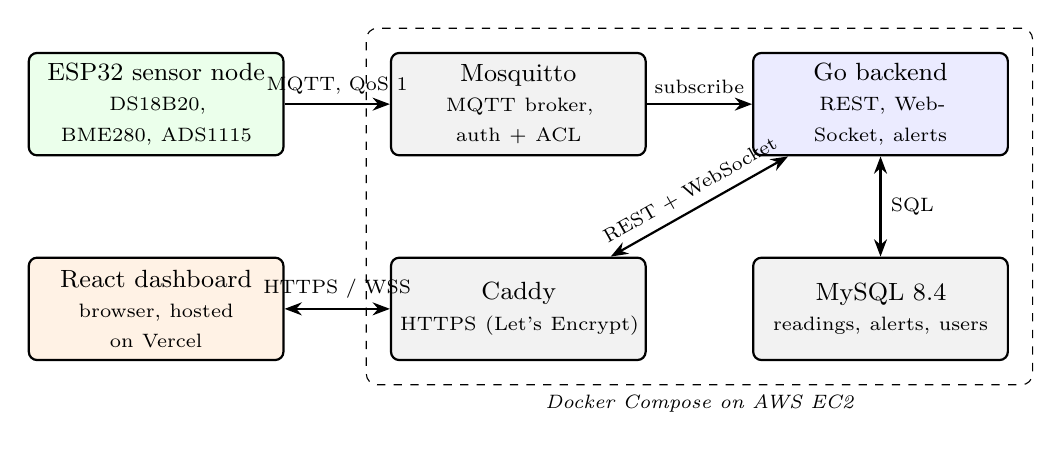
\begin{tikzpicture}[
  box/.style={draw, thick, rounded corners=3pt, align=center, text width=30mm,
              minimum height=13mm, font=\small},
  arr/.style={-{Stealth[length=2.2mm]}, thick},
  biarr/.style={{Stealth[length=2.2mm]}-{Stealth[length=2.2mm]}, thick},
  lab/.style={font=\scriptsize}]
  \node[box, fill=green!8]  (esp)   at (0,0)     {ESP32 sensor node\\ \scriptsize DS18B20, BME280, ADS1115};
  \node[box, fill=gray!10]  (mq)    at (4.6,0)   {Mosquitto\\ \scriptsize MQTT broker, auth + ACL};
  \node[box, fill=blue!8]   (be)    at (9.2,0)   {Go backend\\ \scriptsize REST, WebSocket, alerts};
  \node[box, fill=gray!10]  (db)    at (9.2,-2.6){MySQL 8.4\\ \scriptsize readings, alerts, users};
  \node[box, fill=gray!10]  (caddy) at (4.6,-2.6){Caddy\\ \scriptsize HTTPS (Let's Encrypt)};
  \node[box, fill=orange!10](ui)    at (0,-2.6)  {React dashboard\\ \scriptsize browser, hosted on Vercel};
  \draw[arr]   (esp) -- node[lab, above]{MQTT, QoS 1} (mq);
  \draw[arr]   (mq)  -- node[lab, above]{subscribe} (be);
  \draw[biarr] (be)  -- node[lab, right]{SQL} (db);
  \draw[biarr] (be)  -- node[lab, above, sloped]{REST + WebSocket} (caddy);
  \draw[biarr] (ui)  -- node[lab, above]{HTTPS / WSS} (caddy);
  \node[draw, dashed, rounded corners, inner sep=3mm, fit=(mq)(be)(db)(caddy)] (dock) {};
  \node[font=\scriptsize\itshape, anchor=north] at (dock.south) {Docker Compose on AWS EC2};
\end{tikzpicture}
\end{adjustbox}
\caption{High-level architecture of the PulsePonics platform}
\label{fig:arch}
\end{figure}

\section{Technology Stack}
Table~\ref{tab:stack} lists the technologies used in each layer. Go was chosen for the
backend for its low memory footprint on a small cloud instance and its first-class
concurrency, which suits a service that runs an MQTT consumer, an HTTP server and
many WebSocket writers at the same time.

\begin{table}[htbp]
\centering
\caption{Technology stack used in the project}
\label{tab:stack}
\small
\begin{tabularx}{\linewidth}{@{}lX@{}}
\toprule
\textbf{Layer} & \textbf{Technology} \\
\midrule
Edge device    & ESP32 (C++, Arduino framework, PlatformIO); DS18B20, ADS1115, BME280 \\
Transport      & MQTT 3.1.1 over TCP; Eclipse Mosquitto 2 with password file and ACL \\
Backend        & Go (standard \code{net/http} router), sqlx, Eclipse Paho MQTT, gorilla/websocket, golang-jwt, bcrypt \\
Database       & MySQL 8.4 (InnoDB), embedded versioned SQL migrations \\
Frontend       & React 19, TypeScript, Vite, Tailwind CSS 4, React Router, Recharts \\
Infrastructure & Docker Compose, Caddy 2 (automatic HTTPS), AWS EC2, Vercel \\
Testing        & \code{go test} with race detector, Vitest, Unity (firmware), Bash end-to-end suite \\
\bottomrule
\end{tabularx}
\end{table}

\section{Data Model}
\label{sec:datamodel}
The schema (Table~\ref{tab:schema}) has six tables. All timestamps are stored in UTC:
the database session and the driver are both pinned to UTC, so the data does not shift
when the server's time zone changes. Every child table references its device with
\code{ON DELETE CASCADE}, so deleting a device or an account removes its data
completely. Two constraints carry business rules directly in the database:
\code{UNIQUE(device\_id, recorded\_at)} on \code{readings} makes ingestion idempotent,
and on \code{alerts} a generated column \code{open\_marker} (1 while the alert is open,
\code{NULL} once resolved) is part of a unique key with device and metric. Because
\code{NULL}s never collide in a unique index, this allows at most one \emph{open} alert
per device and metric while keeping any number of resolved ones.

\begin{table}[htbp]
\centering
\caption{Database schema overview}
\label{tab:schema}
\small
\begin{tabularx}{\linewidth}{@{}l X X@{}}
\toprule
\textbf{Table} & \textbf{Key columns and constraints} & \textbf{Purpose} \\
\midrule
\code{users}          & unique email, bcrypt password hash & user accounts \\
\code{refresh\_tokens} & SHA-256 token hash (unique), expiry, revoked, rotated flag & session rotation and reuse detection \\
\code{devices}        & unique \code{device\_id}, owner FK, API-key hash & device registry and ownership \\
\code{readings}       & six nullable DECIMAL sensors, \code{recorded\_at}; unique (device, time) & telemetry time series \\
\code{thresholds}     & PK (device, metric), min, max, enabled & per-device alert limits \\
\code{alerts}         & metric, kind, trigger/latest value, opened/resolved/acknowledged & alert history \\
\bottomrule
\end{tabularx}
\end{table}



\section{Authentication and Authorization Design}
Users sign up with an email and password, stored as a bcrypt hash~\cite{owaspauth}.
Login returns a pair of tokens:
\begin{itemize}
  \item a \textbf{15-minute access token}: an HS256-signed JWT~\cite{rfc7519},
        sent as a bearer token and checked without a database lookup;
  \item a \textbf{7-day refresh token}: an opaque random string, stored only as its
        SHA-256 hash.
\end{itemize}
Each refresh rotates the token. If a token that has already been rotated is presented
again, it must have been copied, so every session of that user is revoked. A password
change likewise revokes all other sessions.

Authorization is ownership-based. Every device belongs to exactly one user, and every
device-scoped query checks it. Another user's device returns \code{404} rather than
\code{403}, so device IDs cannot be probed.

Devices authenticate separately:
\begin{itemize}
  \item to the broker with an MQTT username and password, restricted by an ACL to
        publishing on \code{hydroponics/+/telemetry} and \code{.../status};
  \item for HTTP ingestion, with a per-device API key that is stored hashed and shown
        only once.
\end{itemize}
Login and signup are rate-limited per IP address, and browser access is restricted to an
allowlist of origins, both for REST calls (CORS) and for WebSocket upgrades.

\section{Telemetry Ingestion Pipeline}
Figure~\ref{fig:seq} traces one reading through the system. MQTT QoS~1 guarantees
\emph{at-least-once} delivery: the firmware re-sends a reading when the broker's
acknowledgment (PUBACK) is late, so the same reading can arrive twice. The backend
makes this safe by relying on the unique \code{(device\_id, recorded\_at)} key. A
duplicate is logged and dropped, and is neither broadcast nor evaluated for alerts.
Readings from device IDs that no user has registered are discarded, and a message whose
payload \code{device\_id} differs from its topic is rejected. A device can therefore
only write its own data.

\begin{figure}[htbp]
\centering
\begin{adjustbox}{max width=\linewidth}
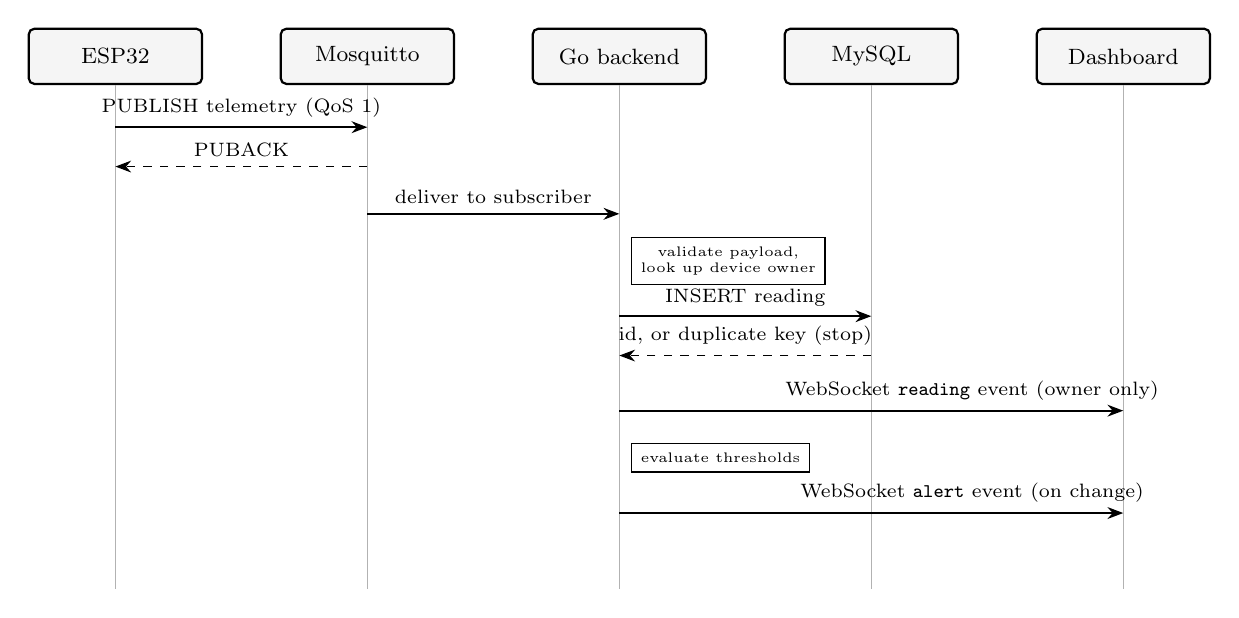
\begin{tikzpicture}[font=\scriptsize,
  actor/.style={draw, thick, rounded corners=2pt, fill=gray!8, minimum width=22mm,
                minimum height=7mm, align=center, font=\footnotesize},
  msg/.style={-{Stealth[length=2mm]}, thick},
  ret/.style={-{Stealth[length=2mm]}, dashed},
  act/.style={draw, fill=white, align=center, font=\tiny, anchor=west}]
  \foreach \x/\nm/\lbl in {0/esp/ESP32, 3.2/mq/Mosquitto, 6.4/be/Go backend, 9.6/db/MySQL, 12.8/ui/Dashboard} {
    \node[actor] (\nm) at (\x,0) {\lbl};
    \draw[gray!60] (\nm.south) -- ++(0,-6.4);
  }
  \draw[msg] (0,-0.9)   -- node[above]{PUBLISH telemetry (QoS 1)} (3.2,-0.9);
  \draw[ret] (3.2,-1.4) -- node[above]{PUBACK} (0,-1.4);
  \draw[msg] (3.2,-2.0) -- node[above]{deliver to subscriber} (6.4,-2.0);
  \node[act] at (6.55,-2.6) {validate payload,\\look up device owner};
  \draw[msg] (6.4,-3.3)  -- node[above]{INSERT reading} (9.6,-3.3);
  \draw[ret] (9.6,-3.8)  -- node[above]{id, or duplicate key (stop)} (6.4,-3.8);
  \draw[msg] (6.4,-4.5)  -- node[above, pos=0.7]{WebSocket \code{reading} event (owner only)} (12.8,-4.5);
  \node[act] at (6.55,-5.1) {evaluate thresholds};
  \draw[msg] (6.4,-5.8)  -- node[above, pos=0.7]{WebSocket \code{alert} event (on change)} (12.8,-5.8);
\end{tikzpicture}
\end{adjustbox}
\caption{Sequence of a telemetry reading from the ESP32 to the dashboard}
\label{fig:seq}
\end{figure}

\section{Alerting Engine Design}
Each device has a minimum and maximum per metric. Defaults are pH 5.5--6.5, EC
1.2--2.4\,mS/cm, water 18--24\degC, air 18--28\degC and humidity 45--75\,\%;
pressure is monitored without limits. The user can edit any of these. Every new
reading is checked against these limits, and an alert moves through two states
(Figure~\ref{fig:alertfsm}).

A naive rule (``resolve as soon as the value is back in range'') makes a noisy sensor
sitting on a limit open and close an alert on every reading. The engine therefore applies
\emph{hysteresis}: an alert resolves only once the value is back inside the band by a
margin of $\alpha = 5\,\%$ of the band's width. For a high-side alert the resolve
condition is
\begin{equation}
  v \;\le\; v_{\max} - \alpha\,(v_{\max} - v_{\min}), \qquad \alpha = 0.05,
  \label{eq:hyst}
\end{equation}
and symmetrically for a low-side alert. A \code{null} sensor value leaves the alert
unchanged, because a missing reading is not evidence that the fault has cleared.

\begin{figure}[htbp]
\centering
\begin{adjustbox}{max width=\linewidth}
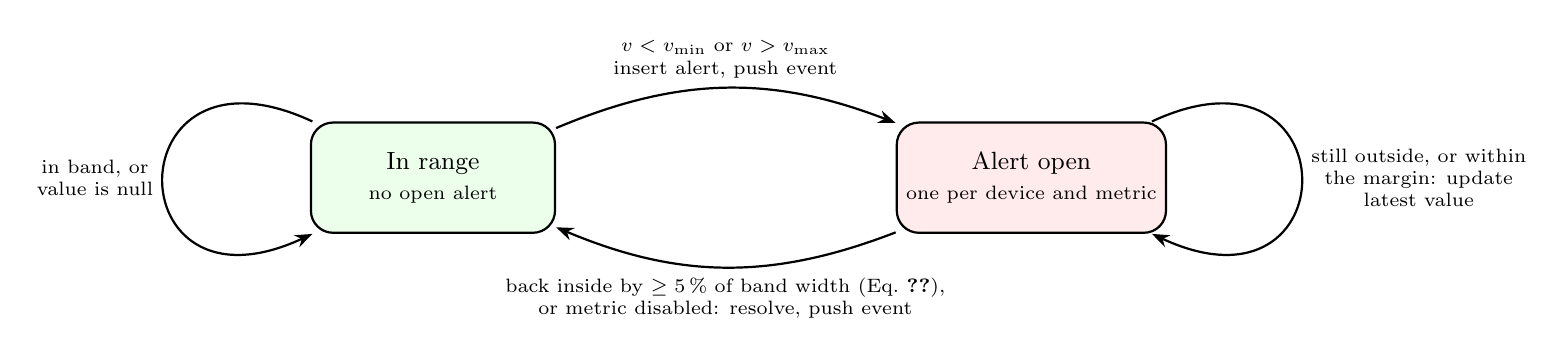
\begin{tikzpicture}[
  st/.style={draw, thick, rounded corners=8pt, minimum width=31mm, minimum height=14mm,
             align=center, font=\small},
  arr/.style={-{Stealth[length=2.2mm]}, thick},
  lab/.style={font=\scriptsize, align=center}]
  \node[st, fill=green!8] (ok)   at (0,0)   {In range\\ \scriptsize no open alert};
  \node[st, fill=red!8]   (open) at (7.6,0) {Alert open\\ \scriptsize one per device and metric};
  \draw[arr] (ok) to[bend left=22]
      node[lab, above]{$v < v_{\min}$ or $v > v_{\max}$\\insert alert, push event} (open);
  \draw[arr] (open) to[bend left=22]
      node[lab, below]{back inside by $\ge 5\,\%$ of band width (Eq.~\ref{eq:hyst}),\\or metric disabled: resolve, push event} (ok);
  \draw[arr] (open) to[out=25, in=-25, looseness=5]
      node[lab, right]{still outside, or within\\the margin: update\\latest value} (open);
  \draw[arr] (ok) to[out=155, in=205, looseness=5]
      node[lab, left]{in band, or\\value is null} (ok);
\end{tikzpicture}
\end{adjustbox}
\caption{Alert state machine with hysteresis (per device and metric)}
\label{fig:alertfsm}
\end{figure}

\section{Time-Series Query Strategy}
At the firmware's development interval of 10\,s, a device produces 8,640 readings per
day, far more than a chart needs and slow to send to a phone. The history endpoint
therefore returns at most $N$ points (default 500). If the requested range $R$ contains
more readings than that, MySQL averages them into epoch-aligned buckets of size
\begin{equation}
  b = \min\left\{\, s \in S \;:\; s \ge \left\lceil \tfrac{R}{N-1} \right\rceil \right\},
  \quad S = \{10, 15, 30, 60, 120, 300, \dots, 86400\}\ \text{s}.
  \label{eq:bucket}
\end{equation}
Dividing by $N-1$ instead of $N$ accounts for a range that straddles one extra
epoch-aligned bucket, so the result never exceeds $N$ points. Choosing $b$ from a set of
round values keeps chart timestamps on whole minutes.

% =====================================================================
\chapter{System Implementation}

\section{Backend Structure and API Design}
The backend is organised in vertical feature slices (\code{auth}, \code{devices},
\code{readings}, \code{alerts}), each with its own model, repository, service and HTTP
handler. Shared platform packages provide typed errors, JSON helpers, middleware,
database access, migrations and the WebSocket hub. Services return typed errors that a
single helper maps to HTTP status codes, so internal details never leak to clients.
Table~\ref{tab:endpoints} summarises the 24 routes; all of them are under \code{/api}.

\begin{table}[htbp]
\centering
\caption{Summary of implemented API endpoint categories}
\label{tab:endpoints}
\small
\begin{tabularx}{\linewidth}{@{}l c X@{}}
\toprule
\textbf{Category} & \textbf{Routes} & \textbf{Purpose} \\
\midrule
Authentication and account & 7 & signup, login, refresh, logout, profile, change password, delete account \\
Device registry            & 6 & list, register, get, rename, delete, rotate API key \\
Readings                   & 5 & HTTP ingestion (device key), auto-aggregated history, latest, recent, metric metadata \\
Thresholds and alerts      & 4 & read and update thresholds, list alerts, acknowledge \\
System                     & 2 & health check, authenticated WebSocket stream \\
\midrule
\textbf{Total}             & \textbf{24} & \\
\bottomrule
\end{tabularx}
\end{table}

\section{Input Validation and Data Integrity}
Both ingestion paths (MQTT and HTTP) call the same \code{Ingest} service, which starts
with the validation in Listing~\ref{lst:validate}. The accepted ranges mirror the
firmware's own limits. The firmware already sends out-of-range values as \code{null},
so genuine readings are never rejected while corrupted ones are. A timestamp more than
five minutes in the future, which indicates an unsynchronised device clock, is
refused; otherwise that reading would remain the ``latest'' forever.

\begin{lstlisting}[language=Go, caption={Payload validation against the hardware contract (\code{readings/validate.go})}, label={lst:validate}]
func validate(in *Input, now time.Time) error {
    if err := devices.ValidateDeviceID(in.DeviceID); err != nil {
        return err // 3-64 chars, no MQTT wildcards or '/'
    }
    any := false
    for _, m := range Metrics { // ranges mirror the firmware's include/config.h
        v := in.value(m.Key)
        if v == nil {
            continue // null = sensor missing, failed or uncalibrated
        }
        any = true
        if *v < m.Min || *v > m.Max {
            return apperr.Invalid(m.Key, fmt.Sprintf("%s must be between %s and %s",
                m.Key, fmtNum(m.Min), fmtNum(m.Max)))
        }
    }
    if !any {
        return apperr.Invalid("", "at least one sensor value must be provided")
    }
    if in.RecordedAt.IsZero() {
        in.RecordedAt = now
    }
    if in.RecordedAt.After(now.Add(maxClockSkew)) { // 5 minutes
        return apperr.Invalid("recorded_at", "recorded_at is in the future; check the device clock")
    }
    in.RecordedAt = in.RecordedAt.UTC().Truncate(time.Millisecond) // matches DATETIME(3)
    return nil
}
\end{lstlisting}

\section{Resilient MQTT Subscription}
With a clean MQTT session, the broker forgets a client's subscriptions when its
connection drops. An early version of the backend subscribed only once at startup. It
reconnected after a broker restart but silently stopped receiving telemetry while
reporting itself healthy. The subscription is therefore issued in the on-connect
handler, which runs after every reconnection (Listing~\ref{lst:mqtt}). Connection retry
is also enabled, so the backend waits for a broker that starts after it instead of
exiting.

\begin{lstlisting}[language=Go, caption={MQTT client set-up and message outcome handling (\code{readings/mqtt\_subscriber.go}, condensed)}, label={lst:mqtt}]
opts := paho.NewClientOptions().
    AddBroker(cfg.BrokerURL).
    SetUsername(cfg.Username).SetPassword(cfg.Password).
    SetAutoReconnect(true).
    SetConnectRetry(true). // keep retrying if the broker is not up yet at boot
    SetConnectRetryInterval(5 * time.Second)

// Subscribe on EVERY (re)connect: a clean session loses subscriptions on disconnect.
opts.SetOnConnectHandler(func(c paho.Client) {
    c.Subscribe("hydroponics/+/telemetry", 1, s.handleMessage)
})

// inside handleMessage, after checking payload device_id == topic device_id:
reading, err := s.service.Ingest(ctx, in)
switch {
case err == nil:
    log.Printf("mqtt: stored reading id=%d device=%s", reading.ID, reading.DeviceID)
case errors.Is(err, ErrUnknownDevice):
    log.Printf("mqtt: device %q is not registered, reading dropped", in.DeviceID)
case errors.Is(err, ErrDuplicate):
    log.Printf("mqtt: duplicate reading device=%s ignored (firmware retry)", in.DeviceID)
default:
    log.Printf("mqtt: rejected reading from %s: %v", in.DeviceID, err)
}
\end{lstlisting}

\section{Alert Decision Logic}
The state machine of Figure~\ref{fig:alertfsm} is implemented as a pure function
(Listing~\ref{lst:decide}) that is exhaustively unit-tested. A thin service layer turns
its decision into database writes and WebSocket events. If two readings race to open the
same alert, the unique \code{open\_marker} key described in Section~\ref{sec:datamodel}
rejects the second insert.

\begin{lstlisting}[language=Go, caption={Alert decision with hysteresis (\code{alerts/thresholds.go}, condensed)}, label={lst:decide}]
func decide(t Threshold, value float64, open *Alert) decision {
    if !t.Enabled {
        if open != nil {
            return decision{action: actionResolve}
        }
        return decision{action: actionNone}
    }
    var breached decision
    switch {
    case t.Min != nil && value < *t.Min:
        breached = decision{kind: "low", bound: *t.Min}
    case t.Max != nil && value > *t.Max:
        breached = decision{kind: "high", bound: *t.Max}
    }
    if breached.kind != "" {
        breached.action = actionOpen
        if open != nil {
            breached.action = actionUpdate
        }
        return breached
    }
    if open == nil {
        return decision{action: actionNone}
    }
    margin := 0.0
    if t.Min != nil && t.Max != nil {
        margin = (*t.Max - *t.Min) * hysteresisFraction // 0.05
    }
    if (open.Kind == "low" && t.Min != nil && value < *t.Min+margin) ||
        (open.Kind == "high" && t.Max != nil && value > *t.Max-margin) {
        return decision{action: actionUpdate, kind: open.Kind, bound: open.ThresholdValue}
    }
    return decision{action: actionResolve}
}
\end{lstlisting}

\section{Time-Bucketed Aggregation}
The downsampling of Equation~\ref{eq:bucket} runs inside MySQL (Listing~\ref{lst:agg}),
so only the averaged points cross the network. The service first counts the readings in
the range, using the index on \code{(device\_id, recorded\_at)}. If the count fits within
$N$, it returns raw readings; otherwise it runs the aggregate query with the chosen
bucket size.

\begin{lstlisting}[language=SQL, caption={Server-side aggregation of a history range into fixed buckets}, label={lst:agg}]
SELECT FROM_UNIXTIME(FLOOR(UNIX_TIMESTAMP(recorded_at) / ?) * ?) AS recorded_at,
       AVG(ph) AS ph, AVG(ec_ms_cm) AS ec_ms_cm, AVG(water_temp_c) AS water_temp_c,
       AVG(air_temp_c) AS air_temp_c, AVG(humidity_pct) AS humidity_pct,
       AVG(pressure_hpa) AS pressure_hpa
FROM readings
WHERE device_id = ? AND recorded_at >= ? AND recorded_at <= ?
GROUP BY 1
ORDER BY 1;
\end{lstlisting}

\section{Real-Time Delivery}
The WebSocket hub keeps connections grouped by user. Publishing an event never touches
the network directly. Each client has a buffered queue of 64 messages, drained by its own
writer goroutine with a 10\,s write deadline, and a client whose queue is full is
disconnected instead of being allowed to stall ingestion. The server pings every 54\,s
and drops clients that do not answer, which removes half-open connections left behind by
a mobile browser that lost signal. Browsers cannot set headers on a WebSocket request,
so the short-lived access token is passed as a query parameter and verified once, at
connect time.

\section{Frontend Dashboard}
The dashboard is a single-page React application with six routes: sign in, sign up,
device list, device dashboard, device settings and account. One authenticated WebSocket
per tab feeds every page. New readings update the cards, chart and table in place, and
after a reconnect each page refetches its data to fill in anything it missed. Pages load
data through a small hook that aborts superseded requests, so switching devices can never
show another device's data.

The access token is held only in memory. The refresh token is kept in
\code{localStorage}, because the API and the dashboard are on different sites, where
third-party cookies are unreliable. Since refresh tokens are single-use, two browser tabs
must never refresh with the same token. Refreshes are therefore serialised across tabs
with the Web Locks API, re-reading the current token inside the lock
(Listing~\ref{lst:refresh}).

\begin{lstlisting}[language=TypeScript, caption={Cross-tab-safe session refresh (\code{lib/session.ts}, condensed)}, label={lst:refresh}]
export function refreshSession(): Promise<Session | null> {
  if (!inflight) {
    // one refresh at a time, across all open tabs
    inflight = navigator.locks.request('pulseponics-refresh', async () => {
      const token = readRefreshToken() // re-read: another tab may have rotated it
      if (!token) { clearSession(); return null }
      const res = await fetch(apiUrl('/api/auth/refresh'), {
        method: 'POST',
        headers: { 'Content-Type': 'application/json' },
        body: JSON.stringify({ refresh_token: token }),
      })
      if (res.status === 401) { clearSession(); return null }
      const session = (await res.json()) as Session
      setSession(session) // store the rotated refresh token
      return session
    }).finally(() => { inflight = null })
  }
  return inflight
}
\end{lstlisting}

\section{Containerisation and Deployment}
The stack is defined in a single Docker Compose file with five services: MySQL and the
backend are bound to localhost only, Mosquitto is exposed on port 1883 for the devices,
Caddy (port 80/443) is enabled by the \code{prod} profile, and the simulator by the
\code{sim} profile. The backend starts only after the database and broker pass their
health checks, and Mosquitto's password file and ACL are generated from environment
variables when its container starts. One command, \code{docker compose up}, starts the
stack locally. On EC2, Caddy obtains and renews a TLS certificate for an \code{sslip.io}
hostname derived from the instance's Elastic IP, so no domain purchase is
needed~\cite{caddy}. The backend image is built in two stages and runs as a non-root
user. Database migrations are embedded in the binary and applied at startup. MySQL is
tuned to fit a 1\,GB t3.micro instance. The frontend is deployed separately on Vercel.

\section{Testing and Quality Assurance}
\label{sec:testing}
Testing was carried out at three levels:
\begin{itemize}
  \item \textbf{Unit tests} cover the pure logic: Go tests with the race detector for
        the backend, Vitest for the dashboard's helper functions, and the firmware's
        conversion maths on the host machine.
  \item \textbf{An end-to-end suite} (\code{scripts/smoke-test.sh}) drives the live
        containerised stack through 38 checks: real MQTT publishes with the exact
        firmware payload, duplicates, unregistered devices, wrong broker passwords,
        alerts, threshold changes, isolation between users, WebSocket delivery, CORS
        and session rotation.
  \item \textbf{Static analysis} with \code{go vet}, \code{gofmt}, ESLint (including
        React's hook-purity rules) and strict TypeScript.
\end{itemize}

% =====================================================================
\chapter{Result}

\section{Summary of Deliverables}
\begin{table}[htbp]
\centering
\caption{Summary of key results achieved}
\label{tab:results}
\small
\begin{tabularx}{\linewidth}{@{}X l@{}}
\toprule
\textbf{Metric} & \textbf{Outcome} \\
\midrule
REST and WebSocket routes implemented                 & 24 \\
Backend code (Go, excluding tests)                    & approx.\ 3,400 lines \\
Frontend code (TypeScript, TSX, CSS)                  & approx.\ 3,000 lines, 6 pages \\
Containerised services                                & 5 (MySQL, Mosquitto, backend, Caddy, simulator) \\
Automated checks passing                              & 106 (48 backend, 8 frontend, 12 firmware, 38 end-to-end) \\
Median HTTP ingestion latency                         & 2.6\,ms \\
Median MQTT-to-dashboard latency                      & 1.9\,ms \\
Duplicate readings stored after a PUBACK retry        & 0 (3 publishes $\rightarrow$ 1 row) \\
Recovery after a broker restart                       & automatic, about 1\,s \\
\bottomrule
\end{tabularx}
\end{table}

All measurements in this chapter were taken on the development machine (Apple Silicon
laptop, Docker Desktop), with the client and the stack on the same host. Network latency
to a cloud server is therefore not included.

\section{Telemetry Visualisation and Alert Behaviour}
To evaluate the pipeline over a realistic period, a six-hour series of 2,160 readings
at the firmware's 10\,s interval was ingested through the HTTP ingestion path. The pH
followed a noisy random walk around 6.0, water temperature followed a slow daily swing,
and a pH dosing fault was injected between 2.5\,h and 3.5\,h, pulling the pH towards 6.9.
Figure~\ref{fig:telemetry} plots the history exactly as the dashboard receives it. The
backend downsampled the 2,160 readings into 361 one-minute averages using
Equation~\ref{eq:bucket}.

The alerting engine opened exactly \textbf{one} pH alert, at $t = 2.58$\,h, when a reading
of 6.54 first exceeded the 6.5 limit. It resolved it at $t = 3.56$\,h, after the value had
fallen below the hysteresis level of 6.45. Although the noisy signal crossed the 6.5
boundary several times while rising and falling, no duplicate or flapping alerts were
produced.

\begin{figure}[htbp]
\centering
\begin{tikzpicture}
\begin{axis}[name=phplot,
  width=\linewidth, height=4.6cm,
  xmin=0, xmax=6, ymin=5.6, ymax=7.2,
  ylabel={pH}, xticklabels={},
  grid=major, grid style={gray!20},
  tick label style={font=\footnotesize}, label style={font=\small},
  legend style={font=\scriptsize, at={(0.01,0.97)}, anchor=north west, draw=gray!50}]
  \fill[green!12] (axis cs:0,5.6) rectangle (axis cs:6,6.5);
  \fill[red!12] (axis cs:2.578,5.6) rectangle (axis cs:3.556,7.2);
  \draw[dashed, orange!70!black, thick] (axis cs:0,6.5) -- (axis cs:6,6.5);
  \addplot[thick, color=brand, mark=none] table[x=hours, y=ph] {data/telemetry_6h.dat};
  \addlegendentry{pH (1-min average)}
  \node[font=\scriptsize, anchor=north] at (axis cs:3.067,7.17) {alert open};
  \node[font=\scriptsize, anchor=south east, orange!70!black] at (axis cs:5.95,6.5) {max 6.5};
\end{axis}
\begin{axis}[at={(phplot.south)}, anchor=north, yshift=-3mm,
  width=\linewidth, height=3.9cm,
  xmin=0, xmax=6, ymin=17.5, ymax=25,
  xlabel={Time (hours)}, ylabel={Water temp. (\textdegree C)},
  grid=major, grid style={gray!20},
  tick label style={font=\footnotesize}, label style={font=\small},
  legend style={font=\scriptsize, at={(0.99,0.97)}, anchor=north east, draw=gray!50}]
  \fill[green!12] (axis cs:0,18) rectangle (axis cs:6,24);
  \addplot[thick, color=blue!60!black, mark=none] table[x=hours, y=water] {data/telemetry_6h.dat};
  \addlegendentry{water temperature (1-min average)}
\end{axis}
\end{tikzpicture}
\caption{Six hours of telemetry as served by the history API (green: threshold band;
red: interval during which the pH alert was open)}
\label{fig:telemetry}
\end{figure}

\section{API and End-to-End Performance}
Each endpoint was called 300 times in sequence against the running stack.
Figure~\ref{fig:latency} reports the median (p50) and 95th-percentile (p95) response
times. Simple lookups complete in 1--2\,ms. A raw one-hour history query, returning 360
readings, takes 3.6\,ms, and aggregating six hours of data inside MySQL takes 6.3\,ms.
End-to-end latency was measured from the moment a reading was published to the broker
until it arrived as a \code{reading} event on an authenticated WebSocket. Over 200
messages it was 1.9\,ms at the median and never more than 4.1\,ms. Login is deliberately
slower (112\,ms median), because bcrypt is designed to be expensive to resist password
guessing; for that reason it is not shown on the chart's scale.

\begin{figure}[htbp]
\centering
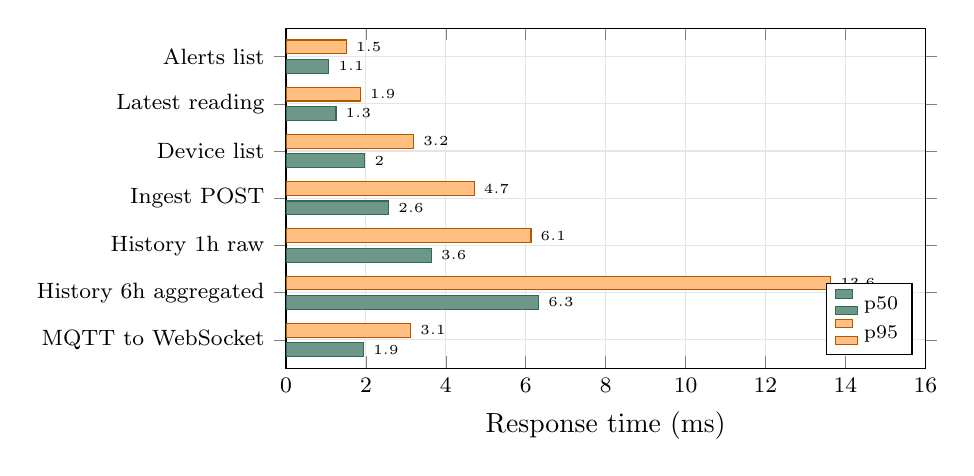
\begin{tikzpicture}
\begin{axis}[
  xbar, width=0.8\linewidth, height=5.9cm,
  bar width=5pt, xmin=0, xmax=16,
  xlabel={Response time (ms)},
  symbolic y coords={MQTT to WebSocket,History 6h aggregated,History 1h raw,Ingest POST,Device list,Latest reading,Alerts list},
  ytick=data, y tick label style={font=\footnotesize}, x tick label style={font=\footnotesize},
  enlarge y limits=0.1,
  point meta=x, nodes near coords,
  every node near coord/.append style={font=\tiny, /pgf/number format/fixed, /pgf/number format/precision=1},
  legend style={font=\scriptsize, at={(0.98,0.04)}, anchor=south east},
  grid=major, grid style={gray!20}]
  \addplot[fill=brand!70, draw=brand] coordinates {
    (1.94,MQTT to WebSocket) (6.32,History 6h aggregated) (3.64,History 1h raw)
    (2.57,Ingest POST) (1.97,Device list) (1.25,Latest reading) (1.07,Alerts list)};
  \addplot[fill=orange!50, draw=orange!70!black] coordinates {
    (3.12,MQTT to WebSocket) (13.63,History 6h aggregated) (6.13,History 1h raw)
    (4.71,Ingest POST) (3.19,Device list) (1.86,Latest reading) (1.51,Alerts list)};
  \legend{p50, p95}
\end{axis}
\end{tikzpicture}
\caption{Measured response times of key operations (300 requests each; 200 messages end to end)}
\label{fig:latency}
\end{figure}

\section{Reliability and Data Integrity}
Several fault scenarios were reproduced against the running stack:
\begin{itemize}
  \item \textbf{Duplicate delivery:} the same reading published three times, as a
        firmware PUBACK retry would, was stored once. The other two were logged as
        duplicates and were neither broadcast nor alerted on.
  \item \textbf{Broker restart:} the backend logged the lost connection, reconnected
        and resubscribed within about one second, and the next reading was stored.
  \item \textbf{Unregistered or spoofed devices:} readings from unregistered IDs, and
        payloads whose \code{device\_id} differed from the topic, were dropped. A
        wrong broker password was refused by Mosquitto.
  \item \textbf{User isolation:} a second account received \code{404} for the first
        account's device, and received none of its WebSocket events.
\end{itemize}

\section{Dashboard}
Figure~\ref{fig:dashboard} shows the device dashboard during a live alert. The pH card
is flagged \emph{Too high}, the chart shows the threshold band, the alert can be
acknowledged, and recent out-of-range values are highlighted. Figure~\ref{fig:ui2} shows
the per-device threshold editor, which gives immediate validation feedback and applies
changes to the latest reading at once, and the responsive layout on a phone.

\begin{figure}[htbp]
\centering
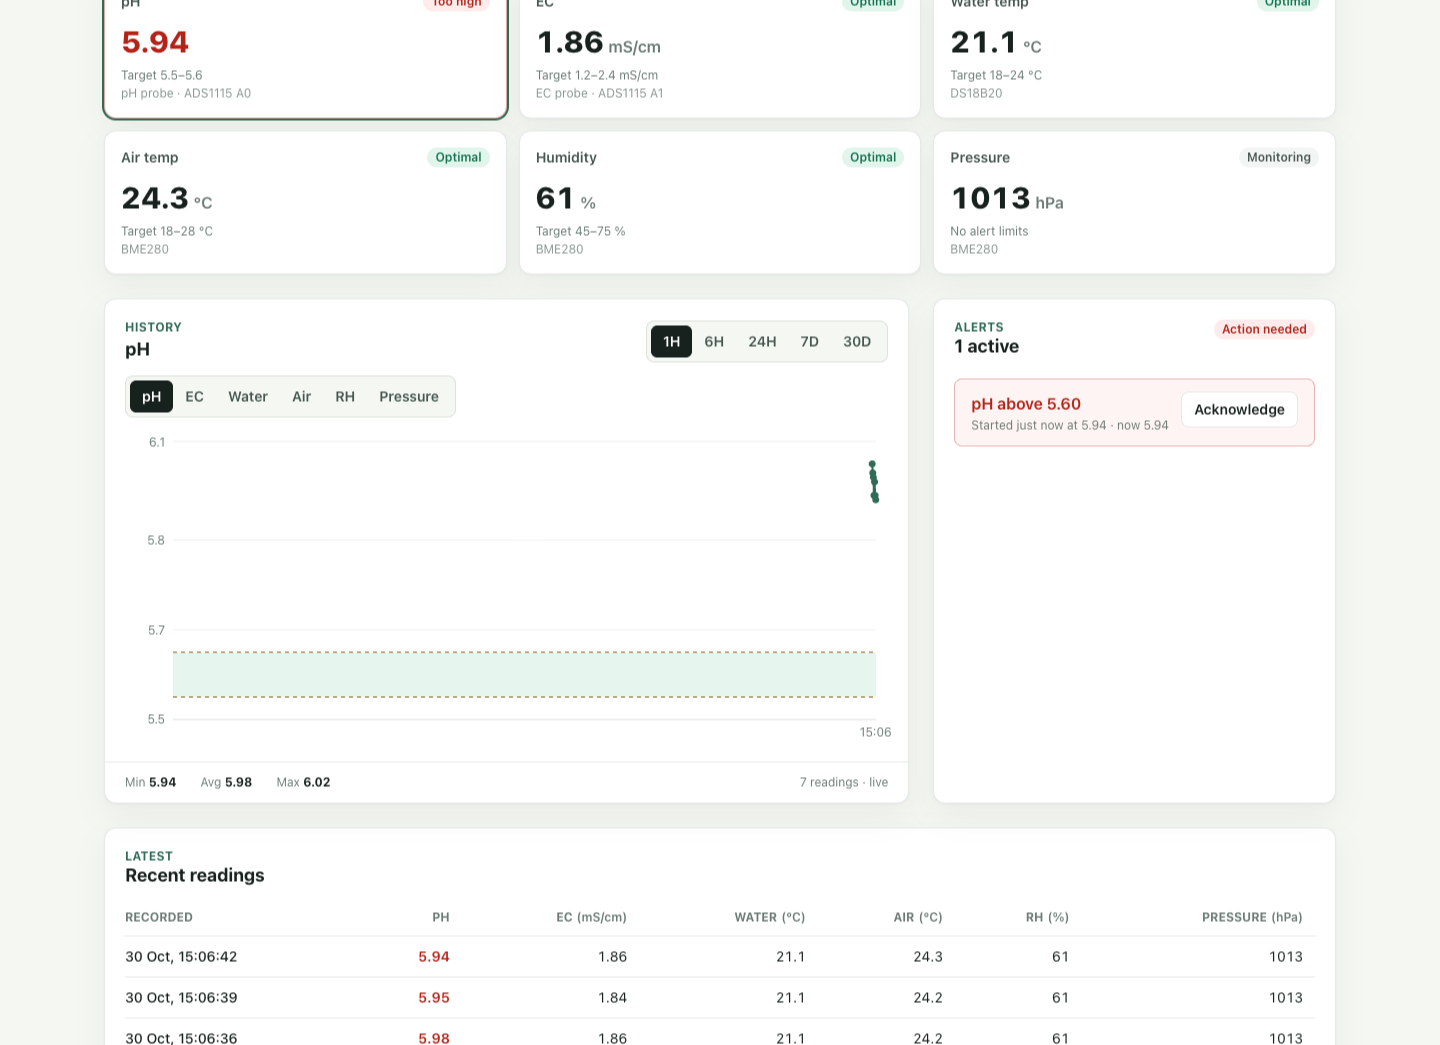
\includegraphics[width=0.84\linewidth]{figures/dashboard.png}
\caption{Device dashboard with live readings, history chart and an open pH alert}
\label{fig:dashboard}
\end{figure}

\begin{figure}[htbp]
\centering
\begin{subfigure}[t]{0.54\linewidth}
  \centering
  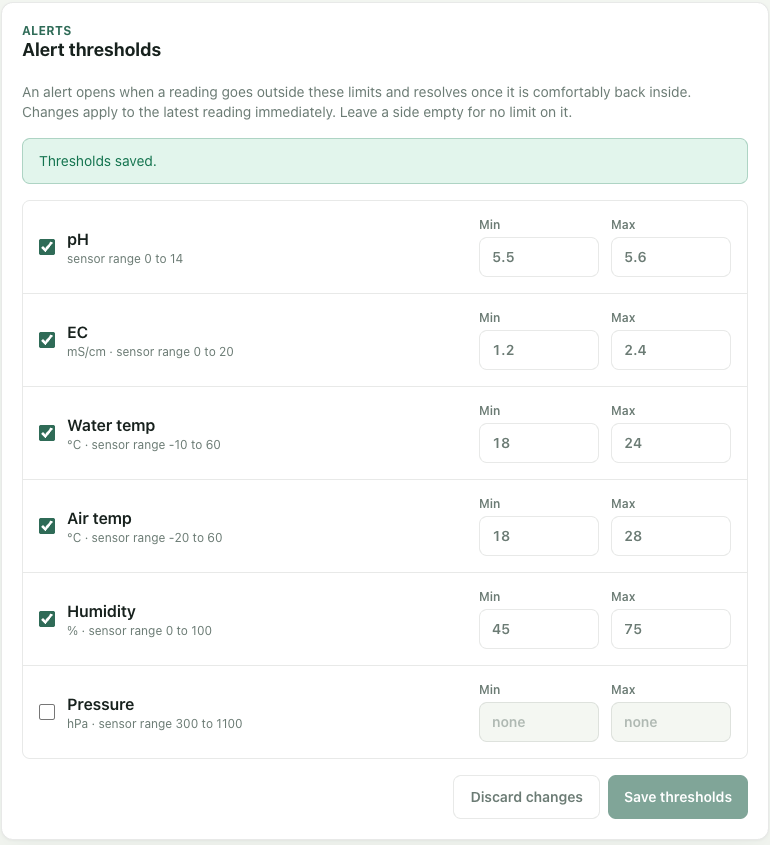
\includegraphics[width=\linewidth]{figures/thresholds.png}
  \caption{Per-device alert threshold editor}
\end{subfigure}\hfill
\begin{subfigure}[t]{0.3\linewidth}
  \centering
  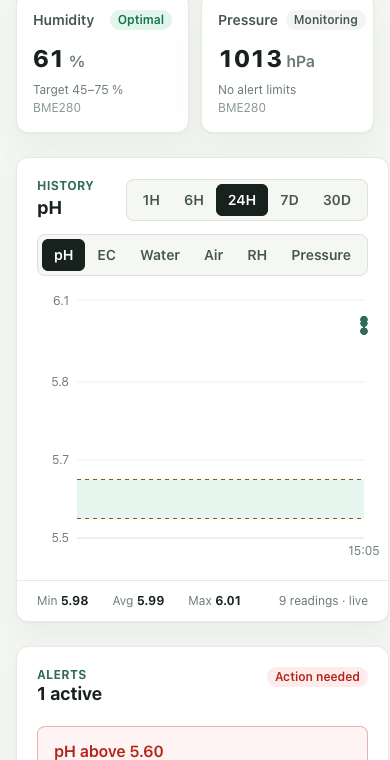
\includegraphics[width=\linewidth]{figures/mobile.png}
  \caption{Mobile layout}
\end{subfigure}
\caption{Threshold configuration and responsive design of the dashboard}
\label{fig:ui2}
\end{figure}

\section{Test Results}
\begin{table}[htbp]
\centering
\caption{Automated test results}
\label{tab:tests}
\small
\begin{tabularx}{\linewidth}{@{}l X c c@{}}
\toprule
\textbf{Suite} & \textbf{Scope} & \textbf{Cases} & \textbf{Result} \\
\midrule
Backend unit       & validation, ingestion flow, bucket sizing, alert decisions and lifecycle, tokens, refresh rotation and reuse, CORS, migrations & 48 & pass \\
Frontend unit      & metric state, formatting, chart gap detection, axis scaling & 8 & pass \\
Firmware unit      & pH/EC conversion, temperature compensation, range checks & 12 & pass \\
End-to-end         & full stack over real MQTT, HTTP and WebSocket (Section~\ref{sec:testing}) & 38 & pass \\
Static analysis    & \code{go vet}, \code{gofmt}, ESLint, strict TypeScript & -- & clean \\
\bottomrule
\end{tabularx}
\end{table}

% =====================================================================
\chapter{Discussion}

\section{Engineering Reliable Ingestion}
The central challenge of the software platform was turning MQTT's at-least-once
delivery and an intermittently connected device into a clean, gap-aware time series.
Three issues surfaced during development, and each was fixed at its root rather than
patched over:
\begin{itemize}
  \item \textbf{Duplicates.} The firmware's retry produced duplicate rows. Instead of
        adding deduplication logic to the service, the natural key
        \code{(device\_id, recorded\_at)} was made unique, which makes the insert itself
        idempotent.
  \item \textbf{Silent loss of subscriptions.} After a broker restart, ingestion
        stopped while the service still appeared healthy. Moving the subscription into
        the on-connect handler fixed it, and the scenario is now part of the
        verification.
  \item \textbf{A reserved-word bug.} Running the database migration in a container
        revealed that \code{last\_value} is a reserved word in MySQL 8. It would have
        failed on the first deployment had it not been tested against the real database
        engine. Migrations were also made re-runnable for this reason.
\end{itemize}

\section{Design Trade-offs Considered}
\begin{itemize}
  \item \textbf{MySQL versus a time-series database.} A dedicated time-series database
        offers built-in downsampling, but MySQL was fixed by the proposal and is
        sufficient at this scale: a composite index plus in-database bucketing keeps
        six-hour queries under 7\,ms.
  \item \textbf{Shared versus per-device broker credentials.} All devices share one MQTT
        login, while ownership is enforced by the backend's registry and its
        topic-to-payload check. Per-device credentials would need the broker's
        dynamic-security plugin, which was not worth the complexity for a single-tank
        deployment.
  \item \textbf{Plain MQTT on port 1883 versus TLS on 8883.} TLS on the ESP32 needs an
        embedded root certificate and costs memory. Password authentication over plain
        TCP was accepted for the demonstration phase and is listed as future work.
  \item \textbf{Refresh token in \code{localStorage} versus an httpOnly cookie.} A
        cookie is better protected against cross-site scripting, but it is unreliable
        across the Vercel and EC2 sites. The risk is reduced by short-lived access tokens
        kept in memory, rotation, and reuse detection.
\end{itemize}

\section{Limitations}
The analog pH and EC probes and the BME280 are not yet integrated, so the data analysed
in this report comes from a simulator that uses the firmware's exact contract, not from
a physical tank. Performance was measured on a single machine without network latency
or concurrent load. Alerts are currently delivered in-app only, and device offline
detection from the MQTT status topic is not yet implemented.

% =====================================================================
\chapter{Conclusion}
The first half of the capstone project has delivered a complete, tested software
platform for real-time hydroponics monitoring:
\begin{itemize}
  \item an authenticated MQTT broker;
  \item a Go backend with secure multi-user accounts, a device registry, idempotent
        ingestion, server-side downsampling, a hysteresis-based alerting engine and a
        real-time WebSocket feed;
  \item a responsive React dashboard;
  \item a containerised deployment with automatic HTTPS.
\end{itemize}
The platform accepts the firmware's existing payload without modification, so the
remaining hardware work plugs directly into it. Measured latencies are in the low
milliseconds, the pipeline remained correct under duplicate delivery, broker restarts
and spoofed devices, and all 106 automated checks pass.

\section{Future Scope}
The plan for the second half of the semester is:
\begin{enumerate}
  \item Implement the ADS1115 and BME280 drivers, and perform two-point calibration of
        the pH (4.00/7.00) and EC (1.413/12.88\,mS/cm) probes with temperature
        compensation.
  \item Deploy the stack on AWS EC2 with the dashboard on Vercel, and run a multi-day
        field trial on a real tank.
  \item Add external notifications (Telegram or email) and debounced offline alerts
        based on the MQTT status topic.
  \item Enable MQTT over TLS (port 8883), and evaluate behaviour under concurrent load
        with multiple devices.
\end{enumerate}

% =====================================================================
\begin{thebibliography}{99}
\phantomsection\addcontentsline{toc}{chapter}{References}
\setlength{\itemsep}{1pt}
\small
\bibitem{resh} H.~M. Resh, \emph{Hydroponic Food Production}, 7th ed. Boca Raton, FL: CRC Press, 2012.
\bibitem{mqtt} OASIS, \emph{MQTT Version 3.1.1}, OASIS Standard, 2014. \url{https://docs.oasis-open.org/mqtt/mqtt/v3.1.1/mqtt-v3.1.1.html}
\bibitem{mosquitto} Eclipse Foundation, \emph{Eclipse Mosquitto Documentation}. \url{https://mosquitto.org/documentation/}
\bibitem{rfc7519} M.~Jones, J.~Bradley and N.~Sakimura, ``JSON Web Token (JWT),'' RFC 7519, IETF, 2015.
\bibitem{rfc6455} I.~Fette and A.~Melnikov, ``The WebSocket Protocol,'' RFC 6455, IETF, 2011.
\bibitem{owaspauth} OWASP Foundation, \emph{Authentication and Session Management Cheat Sheets}. \url{https://cheatsheetseries.owasp.org/}
\bibitem{go} The Go Authors, \emph{The Go Programming Language Documentation}. \url{https://go.dev/doc/}
\bibitem{mysql} Oracle, \emph{MySQL 8.4 Reference Manual}. \url{https://dev.mysql.com/doc/refman/8.4/en/}
\bibitem{react} Meta Open Source, \emph{React Documentation}. \url{https://react.dev/}
\bibitem{docker} Docker Inc., \emph{Docker Compose Documentation}. \url{https://docs.docker.com/compose/}
\bibitem{caddy} Caddy Project, \emph{Automatic HTTPS}. \url{https://caddyserver.com/docs/automatic-https}
\bibitem{dfrobot} DFRobot, \emph{Gravity: Analog pH Sensor/Meter Kit V2 and Analog EC Meter V2 -- Product Wiki}. \url{https://wiki.dfrobot.com/}
\end{thebibliography}

\end{document}
